\documentclass[12pt, a4paper]{article}
\usepackage{../../../myconfig} % Gọi file cấu hình từ ngoài gốc vào

% ==========================================
% BẮT ĐẦU NỘI DUNG TÀI LIỆU
% ==========================================
\begin{document}

% Truyền 3 tham số: {Nhãn cam} {Chữ to chính giữa} {Chữ ở góc phải Header}
\titlebox{Chủ đề: định kì}{Đề kiểm tra định kì lần 6}{Đề định kì}

\textit{\textbf{Phần I: Thí sinh trả lời từ câu 1 đến câu 12, mỗi câu thí sinh chỉ chọn một phương án}}

\vspace{0.5cm}

% --- CÂU 1 ---
\questionLinesManual{0}{1}{Biết \(F(x)\) là một nguyên hàm của hàm số \(f(x)\). Trong các khẳng định sau, khẳng định nào đúng?}{%
    \begin{tasks}(2)
        \task \(\displaystyle\int [f(x) - 1] dx = xF(x) - 1 + C\)
        \task \(\displaystyle\int [f(x) - 1] dx = xF(x) - x + C\)
        \task \(\displaystyle\int [f(x) - 1] dx = F(x) - x + C\)
        \task \(\displaystyle\int [f(x) - 1] dx = F(x) - 1 + C\)
    \end{tasks}
}

% --- CÂU 2 ---
\questionLinesManual{0}{2}{Họ nguyên hàm của hàm số \(f(x) = \sin x + 3e^x\) là}{%
    \begin{tasks}(4)
        \task \(-\cos x - 3e^x + C\)
        \task \(-\cos x + 3e^x + C\)
        \task \(\cos x - 3e^x + C\)
        \task \(\cos x + 3e^x + C\)
    \end{tasks}
}

% --- CÂU 3 ---
\questionLinesManual{0}{3}{Cho \(\displaystyle\int_{0}^{1} f(x) dx = 2\) và \(\displaystyle\int_{0}^{1} g(x) dx = 5\). Khi đó \(\displaystyle\int_{0}^{1} (3f(x) - 2g(x)) dx\) bằng là}{%
    \begin{tasks}(4)
        \task \(-4\)
        \task 16
        \task \(-3\)
        \task 11
    \end{tasks}
}

% --- CÂU 4 ---
\questionLinesManual{0}{4}{Tính thể tích vật thể tròn xoay khi quay hình phẳng giới hạn bởi các đường cong \(y = \sqrt{e^x - x}\), \(y = 0\), \(x = 1\), \(x = 2\) xung quanh trục \(Ox\) là}{%
    \begin{tasks}(4)
        \task \(\pi\left(e^2 - e - \dfrac{3}{2}\right)\)
        \task \(e^2 - e - \dfrac{5}{2}\)
        \task \(\pi\left(e^2 - e - \dfrac{5}{2}\right)\)
        \task \(e^2 - e - \dfrac{3}{2}\)
    \end{tasks}
}

% --- CÂU 5 ---
\questionLinesManual{0}{5}{Diện tích hình phẳng tô đâm trong hình vẽ bên dưới bằng

\begin{center}
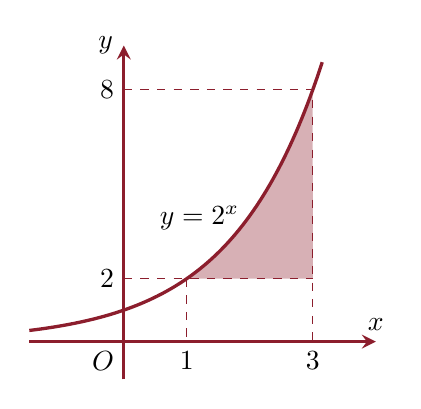
\begin{tikzpicture}[scale=0.8, >=stealth]
    % Định nghĩa màu đỏ đô giống đề bài
    \definecolor{myred}{RGB}{140, 30, 45}

    % Tô màu miền hình phẳng (vùng giữa y = 2^x và y = 2 từ x = 1 đến x = 3)
    % Tỉ lệ tọa độ: x giữ nguyên, y chia cho 2 để hình cân đối
    \fill[myred!35] (1, 1) -- plot[domain=1:3, samples=100] (\x, {2^(\x)/2}) -- (3, 1) -- cycle;

    % Trục tọa độ
    \draw[->, very thick, myred] (-1.5, 0) -- (4.0, 0) node[above, black] {$x$};
    \draw[->, very thick, myred] (0, -0.6) -- (0, 4.7) node[left, black] {$y$};
    
    % Gốc tọa độ O
    \node[below left, black] at (0,0) {$O$};

    % Các đường đứt nét
    \draw[dashed, myred] (0, 4) node[left, black] {$8$} -- (3, 4) -- (3, 0) node[below, black] {$3$};
    \draw[dashed, myred] (0, 1) node[left, black] {$2$} -- (3, 1);
    \draw[dashed, myred] (1, 1) -- (1, 0) node[below, black] {$1$};

    % Đồ thị y = 2^x
    \draw[very thick, myred, domain=-1.5:3.15, samples=100] 
        plot (\x, {2^(\x)/2});

    % Tên đồ thị y = 2^x
    \node[below, black] at (1.2, 2.3) {$y = 2^x$};

\end{tikzpicture}
\end{center}
}{%
    \begin{tasks}(4)
        \task \(\displaystyle\int_{1}^{3} (2^x - 2) dx\)
        \task \(\displaystyle\int_{1}^{3} (2^x + 2) dx\)
        \task \(\displaystyle\int_{1}^{3} (2 - 2^x) dx\)
        \task \(\displaystyle\int_{1}^{3} 2^x dx\)
    \end{tasks}
}

% --- CÂU 6 ---
\questionLinesManual{0}{6}{Cho hàm số \(y = f(x)\) có đạo hàm là \(f'(x)\) liên tục trên \([-2; 3]\). Hàm số \(y = f'(x)\) có đạo hàm như hình vẽ:

\begin{center}
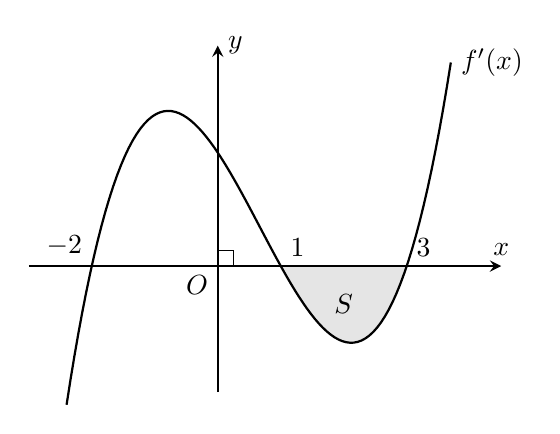
\begin{tikzpicture}[scale=0.8, >=stealth]
    % Tô màu diện tích S dưới trục hoành
    \fill[gray!20] plot[domain=1:3, samples=100] (\x, {0.3*(\x+2)*(\x-1)*(\x-3)}) -- (3,0) -- (1,0) -- cycle;

    % Trục tọa độ
    \draw[->, thick] (-3, 0) -- (4.5, 0) node[above] {$x$};
    \draw[->, thick] (0, -2) -- (0, 3.5) node[right] {$y$};

    % Gốc tọa độ O và ký hiệu góc vuông
    \node[below left] at (0,0) {$O$};
    \draw (0, 0.25) -- (0.25, 0.25) -- (0.25, 0);

    % Đồ thị f'(x) = 0.5*(x+2)*(x-1)*(x-3)
    \draw[thick, domain=-2.4:3.7, samples=100] 
        plot (\x, {0.3*(\x+2)*(\x-1)*(\x-3)}) node[right] {$f'(x)$};

    % Nhãn tọa độ trên trục Ox
    \node[above left] at (-2,0) {$-2$};
    \node[above right] at (1,0) {$1$};
    \node[above right] at (3,0) {$3$};

    % Ký hiệu diện tích S
    \node at (2, -0.6) {$S$};

\end{tikzpicture}
\end{center}

Biết \(\displaystyle\int_{-2}^{1} f'(x) dx = 3\) và diện tích \(S = \dfrac{5}{3}\). Giá trị \(f(3) - f(-2)\) bằng}{%
    \begin{tasks}(4)
        \task \(\dfrac{4}{3}\)
        \task \(-\dfrac{14}{3}\)
        \task \(\dfrac{14}{3}\)
        \task \(-\dfrac{4}{3}\)
    \end{tasks}
}

% --- CÂU 7 ---
\questionLinesManual{0}{7}{Cho \(F(x)\) là nguyên hàm của hàm số \(f(x) = 6x^5 + \dfrac{1}{x^3}\) thỏa mãn \(F(1) = 0\). Tìm \(F(x)\)}{%
    \begin{tasks}(2)
        \task \(F(x) = x^6 - \dfrac{1}{2x^2} + \dfrac{1}{2}\)
        \task \(F(x) = x^6 + \dfrac{1}{2x^2} - \dfrac{3}{2}\)
        \task \(F(x) = x^6 - \dfrac{1}{2x^2} - \dfrac{1}{2}\)
        \task \(F(x) = x^6 - \dfrac{3}{x^2} + 2\)
    \end{tasks}
}

% --- CÂU 8 ---
\questionLinesManual{0}{8}{Biết \(\displaystyle\int g(x) dx = G(x) + C\) (với \(C\) là hằng số). Khi đó khẳng định nào sau đây đúng?}{%
    \begin{tasks}(2)
        \task \(g'(x) = G(x) + C\)
        \task \(G'(x) = g(x)\)
        \task \(G'(x) = g(x) - C\)
        \task \(g'(x) = G(x)\)
    \end{tasks}
}

% --- CÂU 9 ---
\questionLinesManual{0}{9}{Người ta muốn làm một chi tiết máy có dạng khối tròn xoay tạo thành khi quay hình phẳng \(D\) quanh trục \(\Delta\), với \(D\) là hình giới hạn bởi parabol \((P)\) và đường thẳng \(a\), \(\Delta\) là trục đối xứng của \((P)\) (xem hình vẽ minh họa bên). Biết \(a\) cắt \((P)\) tại hai điểm cách nhau 8 cm và khoảng cách từ đỉnh của \((P)\) đến \(a\) bằng 4 cm. Thể tích của chi tiết máy bằng bao nhiêu?

\begin{center}
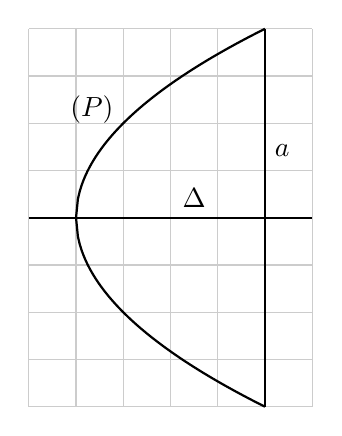
\begin{tikzpicture}[scale=0.6]
    % Lưới ô vuông (Grid 6x8)
    \draw[gray!40, thin] (-1, -4) grid (5, 4);

    % Trục đối xứng \Delta (trục nằm ngang)
    \draw[thick] (-1, 0) -- (5, 0);
    \node[above] at (2.5, 0) {$\Delta$};

    % Đường thẳng a (đường nằm đứng)
    \draw[thick] (4, -4) -- (4, 4);
    \node[right, yshift=-10pt] at (4, 2) {$a$};

    % Parabol (P) có đỉnh tại (0,0), đi qua (4, 4) và (4, -4)
    % Phương trình: x = y^2 / 4  => y = 2*sqrt(x) và y = -2*sqrt(x)
    \draw[thick, domain=0:4, samples=100] plot (\x, {2*sqrt(\x)});
    \draw[thick, domain=0:4, samples=100] plot (\x, {-2*sqrt(\x)});
    
    % Nhãn (P)
    \node[above left] at (1, 1.8) {$(P)$};

\end{tikzpicture}
\end{center}
}{%
    \begin{tasks}(4)
        \task \(4\pi\) cm\(^3\)
        \task \(8\pi\) cm\(^3\)
        \task \(16\pi\) cm\(^3\)
        \task \(32\pi\) cm\(^3\)
    \end{tasks}
}

% --- CÂU 10 ---
\questionLinesManual{0}{10}{Cho hai hàm số \(f(x) = -\dfrac{1}{2}x^3 + \dfrac{3}{2}x^2 + 1\) và \(g(x) = -\dfrac{1}{2}x + \dfrac{5}{2}\) có đồ thị như hình vẽ bên dưới.

\begin{center}
\begin{tikzpicture}[scale=1.0, >=stealth]
    % Định nghĩa màu đỏ đô giống bài toán
    \definecolor{myred}{RGB}{150, 30, 45}

    % Tô màu gạch chéo cho diện tích giữa g(x) và f(x) từ x = -1 đến x = 1
    \fill[pattern=north east lines, pattern color=myred!80] 
        plot[domain=-1:1, samples=100] (\x, {-0.5*\x + 2.5}) -- 
        plot[domain=1:-1, samples=100] (\x, {-0.5*\x*\x*\x + 1.5*\x*\x + 1}) -- cycle;

    % Trục tọa độ
    \draw[->, thick, myred] (-2.0, 0) -- (3.8, 0) node[below, black] {$x$};
    \draw[->, thick, myred] (0, -0.7) -- (0, 5.0) node[left, black] {$y$};

    % Gốc tọa độ O và ký hiệu góc vuông
    \node[below left, black] at (0,0) {$O$};
    \draw[myred] (0, 0.2) -- (0.2, 0.2) -- (0.2, 0);

    % Đường đứt nét (Dashed lines)
    \draw[dashed, myred] (0, 3) node[right, black] {$3$} -- (-1, 3) -- (-1, 0) node[below, black] {$-1$};
    \draw[dashed, myred] (0, 2) node[left, black] {$2$} -- (1, 2) -- (1, 0) node[below, black] {$1$};

    % Đồ thị hàm bậc ba f(x) = -1/2 x^3 + 3/2 x^2 + 1
    \draw[thick, myred, domain=-1.3:3.3, samples=100] 
        plot (\x, {-0.5*\x*\x*\x + 1.5*\x*\x + 1});
    \node[above right, black] at (-1.2, 3.9) {$f(x)$};

    % Đồ thị đường thẳng g(x) = -1/2 x + 5/2
    \draw[thick, myred, domain=-2:3.3, samples=100] 
        plot (\x, {-0.5*\x + 2.5});
    \node[above left, black] at (-2, 3.2) {$g(x)$};

\end{tikzpicture}
\end{center}

Diện tích phần gạch chéo trong hình bằng}{%
    \begin{tasks}(4)
        \task 8
        \task 1
        \task 4
        \task 2
    \end{tasks}
}

% --- CÂU 11 ---
\questionLinesManual{0}{11}{Họ nguyên hàm của hàm số \(f(x) = \sin 2x + \cos 2x\) là}{%
    \begin{tasks}(2)
        \task \(2(-\cos 2x + \sin 2x) + C\)
        \task \(\dfrac{1}{2}(\cos 2x - \sin 2x) + C\)
        \task \(\dfrac{1}{2}(\sin 2x - \cos 2x) + C\)
        \task \(2(\cos 2x - \sin 2x) + C\)
    \end{tasks}
}

% --- CÂU 12 ---
\questionLinesManual{0}{12}{Trong không gian \(Oxyz\), một vật thể được giới hạn bởi hai mặt phẳng \(x = 0\), \(x = 4\). Một mặt phẳng vuông góc với trục \(Ox\) tại điểm có hoành độ bằng \(x\) với \(0 \leq x \leq 4\) cắt vật thể theo mặt cắt là một hình vuông cạnh bằng \(\sqrt{2x + 1}\). Thể tích của vật thể bằng}{%
    \begin{tasks}(4)
        \task \(\dfrac{26}{3}\pi\)
        \task 20
        \task \(20\pi\)
        \task \(\dfrac{26}{3}\)
    \end{tasks}
}
\newpage

\textit{\textbf{Phần II: Thí sinh trả lời từ câu 13 đến câu 16; trong mỗi ý a), b), c), d) ở mỗi câu, thí sinh chọn đúng hoặc sai.}}

\vspace{0.3cm}

% --- CÂU 13 ---
\questionTrueFalse{0}{13}{Một lò sưởi cho trẻ em được lấy ra khỏi tủ lạnh và đặt trên bàn để rã đông. Nhiệt độ của lò sưởi tại thời điểm lấy ra khỏi lạnh là \(-4^\circ C\) và sau \(t\) giờ, tốc độ tăng nhiệt độ của lò sưởi được cho bởi công thức: \(T'(t) = 7e^{-0,35t}\) (\(^\circ C\)/giờ) cho đến khi lò sưởi đạt nhiệt độ môi trường là \(10^\circ C\).}{
    \textbf{a)} & Sau 2 giờ, tốc độ thay đổi nhiệt độ của lò sưởi bằng \(3,48^\circ C\)/giờ (làm tròn kết quả đến hai chữ số thập phân).
    & \textcolor{amberorange}{$\bigcirc$} & \textcolor{amberorange}{$\bigcirc$} \\ \hline
    
    \textbf{b)} & Nhiệt độ lò sưởi tính từ thời điểm lấy ra khỏi tủ lạnh cho đến khi lò sưởi đạt nhiệt độ môi trường được tính bởi công thức \(T(t) = -20e^{-0,35t}\).
    & \textcolor{amberorange}{$\bigcirc$} & \textcolor{amberorange}{$\bigcirc$} \\ \hline
    
    \textbf{c)} & Thời gian để lò sưởi đạt nhiệt độ môi trường là 3,44 giờ (làm tròn kết quả đến hai chữ số thập phân của giờ).
    & \textcolor{amberorange}{$\bigcirc$} & \textcolor{amberorange}{$\bigcirc$} \\ \hline
    
    \textbf{d)} & Ngay sau khi đạt nhiệt độ môi trường, lò sưởi được đưa vào máy hâm sữa. Tốc độ tăng nhiệt độ của lò sưởi trong máy sau \(t\) giờ được xác định bởi: \(L'(t) = ke^{-0,22t}\) (\(k\) là hằng số). Lò sưởi được coi là đạt yêu cầu khi nhiệt độ lò sưởi bằng \(70^\circ\). Biết rằng thời gian cần thiết để hâm nóng lò sưởi là 5 phút thì hằng số \(k \in (720; 730)\).
    & \textcolor{amberorange}{$\bigcirc$} & \textcolor{amberorange}{$\bigcirc$} \\
}

% --- CÂU 14 ---
\questionTrueFalse{0}{14}{Cho một vật đang đứng yên thì bắt đầu chuyển động nhanh dần đều trong khoảng 10 giây với gia tốc là \(a\) (m/s\(^2\)), \(a > 0\). Biết rằng quãng đường vật đi được sau 5 giây kể từ khi bắt đầu chuyển động là 25 m.}{
    \textbf{a)} & Vận tốc của vật tại thời điểm \(t = 5\) (s) là 10 (m/s).
    & \textcolor{amberorange}{$\bigcirc$} & \textcolor{amberorange}{$\bigcirc$} \\ \hline
    
    \textbf{b)} & Vận tốc tức thời của vật là \(v(t) = at\) (m/s).
    & \textcolor{amberorange}{$\bigcirc$} & \textcolor{amberorange}{$\bigcirc$} \\ \hline
    
    \textbf{c)} & \(a = 2\).
    & \textcolor{amberorange}{$\bigcirc$} & \textcolor{amberorange}{$\bigcirc$} \\ \hline
    
    \textbf{d)} & Quãng đường vật đi được sau 10 giây kể từ khi bắt đầu chuyển động là 50 m.
    & \textcolor{amberorange}{$\bigcirc$} & \textcolor{amberorange}{$\bigcirc$} \\
}


% --- CÂU 15 ---
\questionTrueFalse{0}{15}{Một chậu nước có dạng một khối tròn xoay với thiết diện qua trục của chậu (mặt cắt đi qua hai tâm của hai đường tròn đáy) là hai đường parabol đối xứng nhau qua trục đó.

\begin{figure}[H]
    \centering
    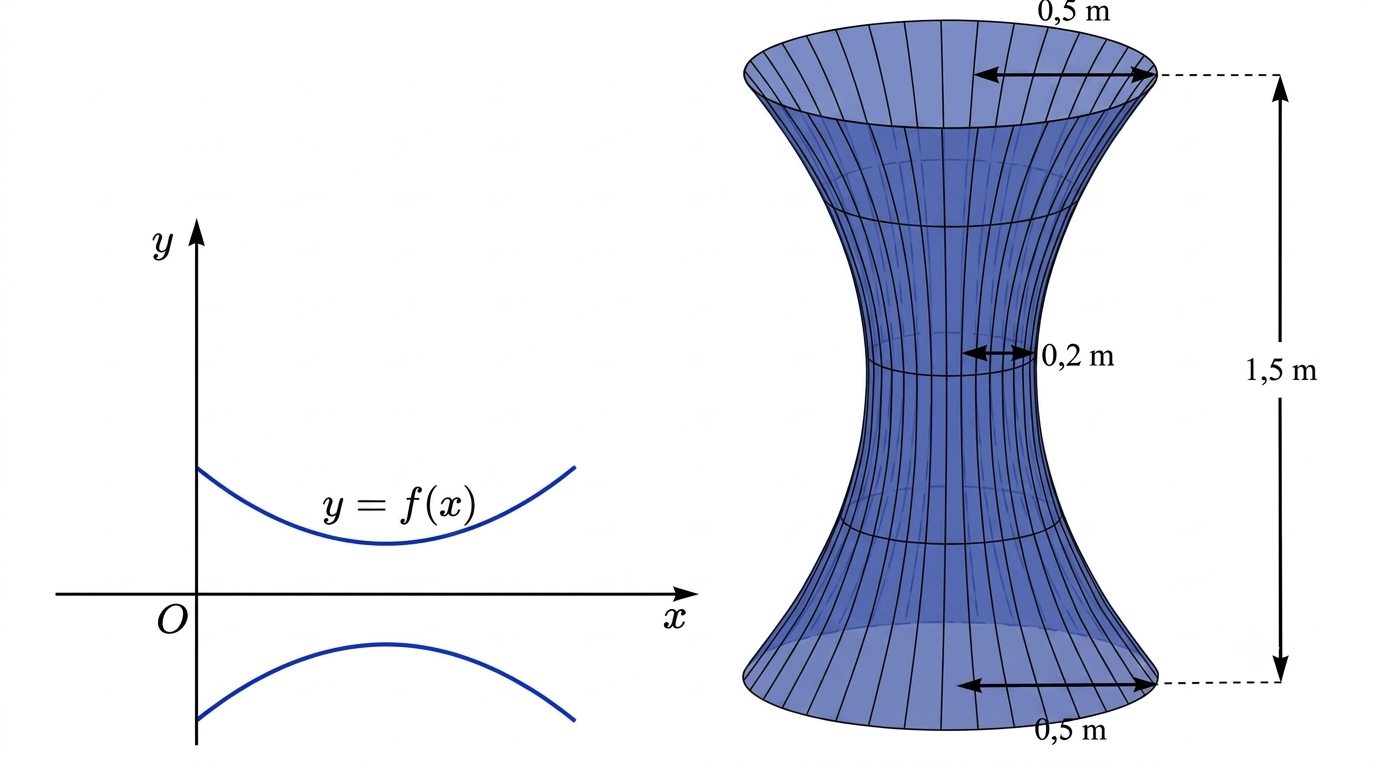
\includegraphics[width=0.7\textwidth]{images/Cau15.png}
\end{figure}

Biết hai đường tròn đáy chậu cùng có bán kính bằng \(0,5\) m; thiết diện nhỏ nhất vuông góc với trục của chậu có bán kính \(0,2\) m; chiều cao của chậu nước bằng \(1,5\) m. Người ta bơm nước vào chậu với tốc độ 5 lít/phút. Xét hệ trục tọa độ \(Oxy\) với gốc \(O\) trùng với tâm đường tròn đáy của chậu nước, tia \(Ox\) chứa trục của chậu nước (đơn vị trên mỗi trục là mét). Mặt cắt qua trục của chậu nước cho ta hai nhánh parabol như hình vẽ. Gọi \(y = f(x)\) là parabol nằm phía trên trục hoành. Xét tính đúng – sai của các mệnh đề sau?}{
    \textbf{a)} & \(f(x) = \dfrac{8}{15}x^2 - \dfrac{4}{5}x + \dfrac{1}{2}\).
    & \textcolor{amberorange}{$\bigcirc$} & \textcolor{amberorange}{$\bigcirc$} \\ \hline
    
    \textbf{b)} & Sức chứa tối đa của chậu nước bằng \(0,5\) m\(^3\) (làm tròn đến hàng phần chục của mét khối).
    & \textcolor{amberorange}{$\bigcirc$} & \textcolor{amberorange}{$\bigcirc$} \\ \hline
    
    \textbf{c)} & Sau 1,5 giờ bơm nước (làm tròn đến hàng phần chục của giờ) thì chậu đầy nước.
    & \textcolor{amberorange}{$\bigcirc$} & \textcolor{amberorange}{$\bigcirc$} \\ \hline
    
    \textbf{d)} & Nếu bơm từ đầu như thế thì đến phút thứ 20, tốc độ dâng lên của nước bằng 0,01 m/phút.
    & \textcolor{amberorange}{$\bigcirc$} & \textcolor{amberorange}{$\bigcirc$} \\
}

% --- CÂU 16 ---
\questionTrueFalse{0}{16}{Đối với ngành nuôi trồng thủy sản, việc kiểm soát lượng thuốc tồn dư trong nước là một nhiệm vụ quan trọng nhằm đáp ứng các tiêu chuẩn an toàn về môi trường. Khi nghiên cứu một loại thuốc trị bệnh trong nuôi trồng thủy sản, người ta sử dụng thuốc đó một lần và theo dõi nồng độ thuốc tồn dư trong nước kể từ lúc sử dụng thuốc. Kết quả cho thấy nồng độ thuốc \(y(t)\) (đơn vị: mg/lít) tồn dư trong nước tại thời điểm \(t\) ngày (\(t \geq 0\)) kể từ lúc sử dụng thuốc, thỏa mãn \(y(t) > 0\) và \(y'(t) = k \cdot y(t)\) (\(t \geq 0\)), trong đó \(k\) là hằng số khác không. Đo nồng độ thuốc tồn dư trong nước tại các thời điểm \(t = 6\) (ngày); \(t = 12\) (ngày) nhận được kết quả lần lượt là 2 mg/lít; 1 mg/lít. Cho biết \(y(t) = e^{g(t)}\) (\(t \geq 0\)).}{
    \textbf{a)} & \(g(t) = kt + C\) (\(t \geq 0\)) với \(C\) là một hằng số xác định.
    & \textcolor{amberorange}{$\bigcirc$} & \textcolor{amberorange}{$\bigcirc$} \\ \hline
    
    \textbf{b)} & \(k = -\dfrac{\ln 2}{3}\).
    & \textcolor{amberorange}{$\bigcirc$} & \textcolor{amberorange}{$\bigcirc$} \\ \hline
    
    \textbf{c)} & \(C = 4\ln 2\).
    & \textcolor{amberorange}{$\bigcirc$} & \textcolor{amberorange}{$\bigcirc$} \\ \hline
    
    \textbf{d)} & Nồng độ thuốc tồn dư trong nước tại thời điểm \(t = 28\) (ngày) kể từ lúc sử dụng thuốc nhỏ hơn \(0,2\) mg/lít.
    & \textcolor{amberorange}{$\bigcirc$} & \textcolor{amberorange}{$\bigcirc$} \\
}

\textit{\textbf{Phần III: Thí sinh trả lời từ câu 17 đến câu 22.}}

\vspace{0.3cm}

% --- CÂU 17 ---
\questionShortAnswer{0}{17}{Ông Duy có một mảnh vườn hình vuông cạnh bằng 8 m. Ông dự định xây một cái bể bơi đặc biệt (phần kẻ sọc trong hình vẽ bên). Biết \(AM = \dfrac{AB}{4}\), phần đường cong đi qua các điểm \(C, M, N\) là một phần của đường Parabol có trục đối xứng là \(MP\) (\(MP \parallel AD\)) và chi phí để làm bể bơi là 5 triệu đồng/1m\(^2\). Số tiền ông Duy phải trả để xây cái bể bơi đó là bao nhiêu triệu đồng? (làm tròn kết quả đến hàng đơn vị).

\begin{center}
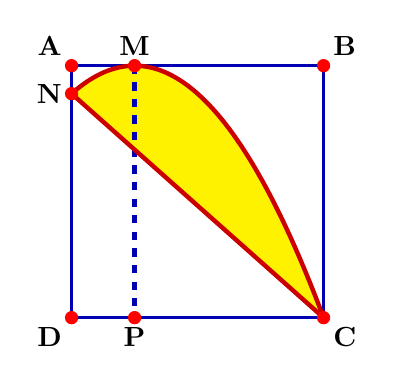
\begin{tikzpicture}[scale=0.8]

    \fill[yellow] plot[domain=0:4, samples=100] (\x, {-4/9*(\x-1)^2 + 4}) -- (0, 32/9) -- cycle;

    % 2. Vẽ hình vuông ABCD
    \draw[very thick, blue!70!black] (0,0) coordinate (D) -- (4,0) coordinate (C) -- (4,4) coordinate (B) -- (0,4) coordinate (A) -- cycle;

    % 3. Vẽ đường thẳng MP (nét đứt)
    \draw[ultra thick, dashed, blue!70!black] (1,4) coordinate (M) -- (1,0) coordinate (P);

    % 4. Vẽ đoạn thẳng NC
    \draw[ultra thick, red!80!black] (0, 32/9) coordinate (N) -- (C);

    % 5. Vẽ Parabol đi qua N, M, C
    \draw[ultra thick, red!80!black, domain=0:4, samples=100] plot (\x, {-4/9*(\x-1)^2 + 4});

    % 6. Vẽ các điểm (nút) màu đỏ
    \fill[red] (A) circle (3pt) node[above left, black] {\textbf{A}};
    \fill[red] (B) circle (3pt) node[above right, black] {\textbf{B}};
    \fill[red] (C) circle (3pt) node[below right, black] {\textbf{C}};
    \fill[red] (D) circle (3pt) node[below left, black] {\textbf{D}};
    \fill[red] (M) circle (3pt) node[above, black] {\textbf{M}};
    \fill[red] (N) circle (3pt) node[left, black] {\textbf{N}};
    \fill[red] (P) circle (3pt) node[below, black] {\textbf{P}};

\end{tikzpicture}
\end{center}
}

% --- CÂU 18 ---
\questionShortAnswer{0}{18}{Một bình hoa có dạng khối tròn xoay với chiều cao là 3 dm. Khi cắt bình hoa theo một mặt phẳng vuông góc với trục của nó thì ta luôn được thiết diện là một hình tròn có bán kính \(y = \sqrt{x^2 - 2x + 2}\) với \(x\) là khoảng cách từ mặt cắt tới mặt đáy của bình hoa, \(x \in [0; 3]\), \(x\) tính theo đơn vị dm. Đổ vào bình một lượng nước để mức nước trong bình cao bằng \(\dfrac{1}{3}\) chiều cao của bình. Hỏi lượng nước này chiếm tỉ lệ bao nhiêu phần trăm so với thể tích của bình hoa, kết quả làm tròn đến hàng đơn vị?
\begin{figure}[H]
    \centering
    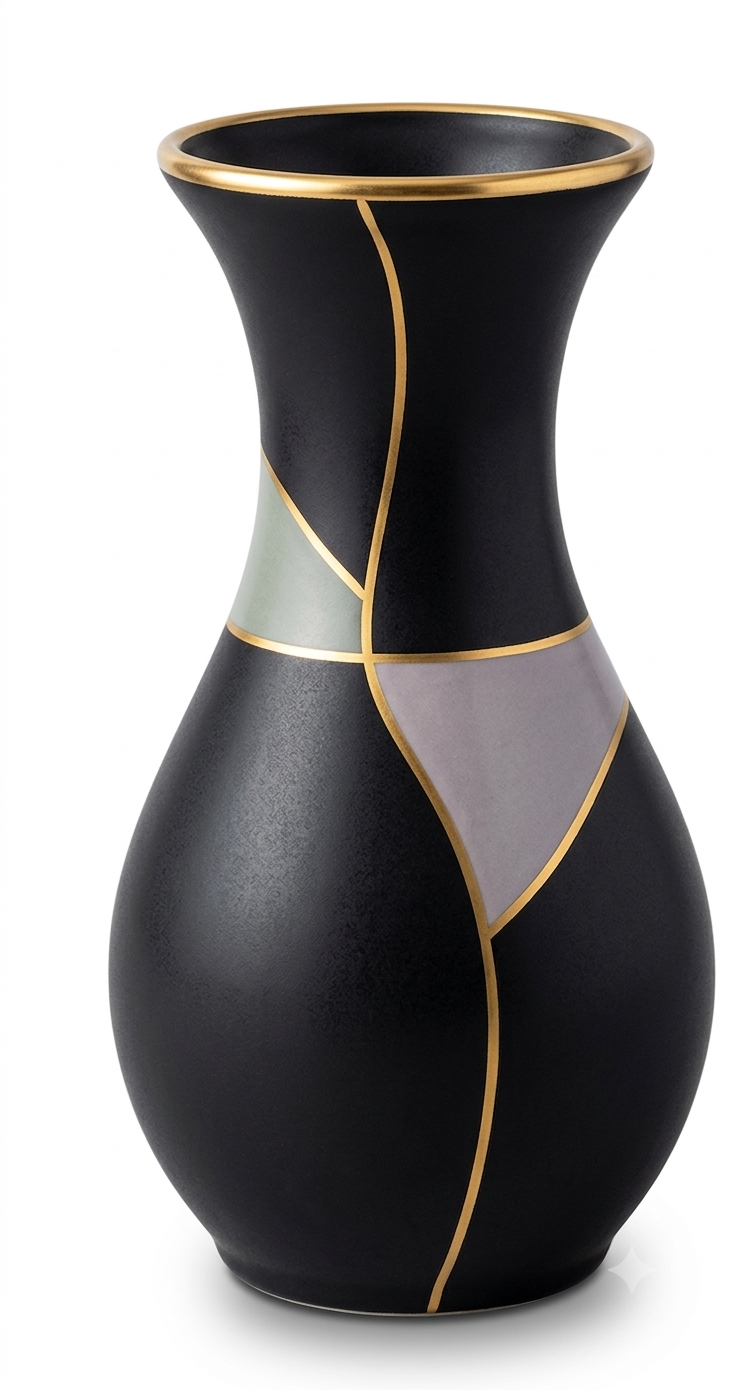
\includegraphics[width=0.1\textwidth]{images/Cau18.png}
\end{figure}
}

% --- CÂU 19 ---
\questionShortAnswer{0}{19}{Một người thiết kế một cái loa phóng thanh bằng nhựa có hình dạng khối tròn xoay như Hình 1 bên dưới, có mặt cắt bởi mặt phẳng qua trục của loa như Hình 2 và có bảng vẽ kỹ thuật trên hệ trục \(Oxy\) như Hình 3 (đơn vị trên các trục bằng 1 cm). Tính thể tích nhựa để đúc chiếc loa (tính theo cm\(^3\) và làm tròn kết quả tính toán sau cùng đến hàng đơn vị).
\begin{figure}[H]
    \centering
    
\includegraphics[width=0.7\textwidth]{images/Cau19.png}
\end{figure}
}

% --- CÂU 20 ---
\questionShortAnswer{0}{20}{Cho vật thể có đáy là hình tròn có bán kính bằng 1 (tham khảo hình vẽ). Khi cắt vật thể bằng mặt phẳng vuông góc với trục \(Ox\) tại điểm có hoành độ \(x\) (\(-1 \leq x \leq 1\)) thì được thiết diện là một tam giác đều. Thể tích \(V\) của vật thể đó là bao nhiêu? (làm tròn đến hàng phần trăm)

\begin{figure}[H]
    \centering
    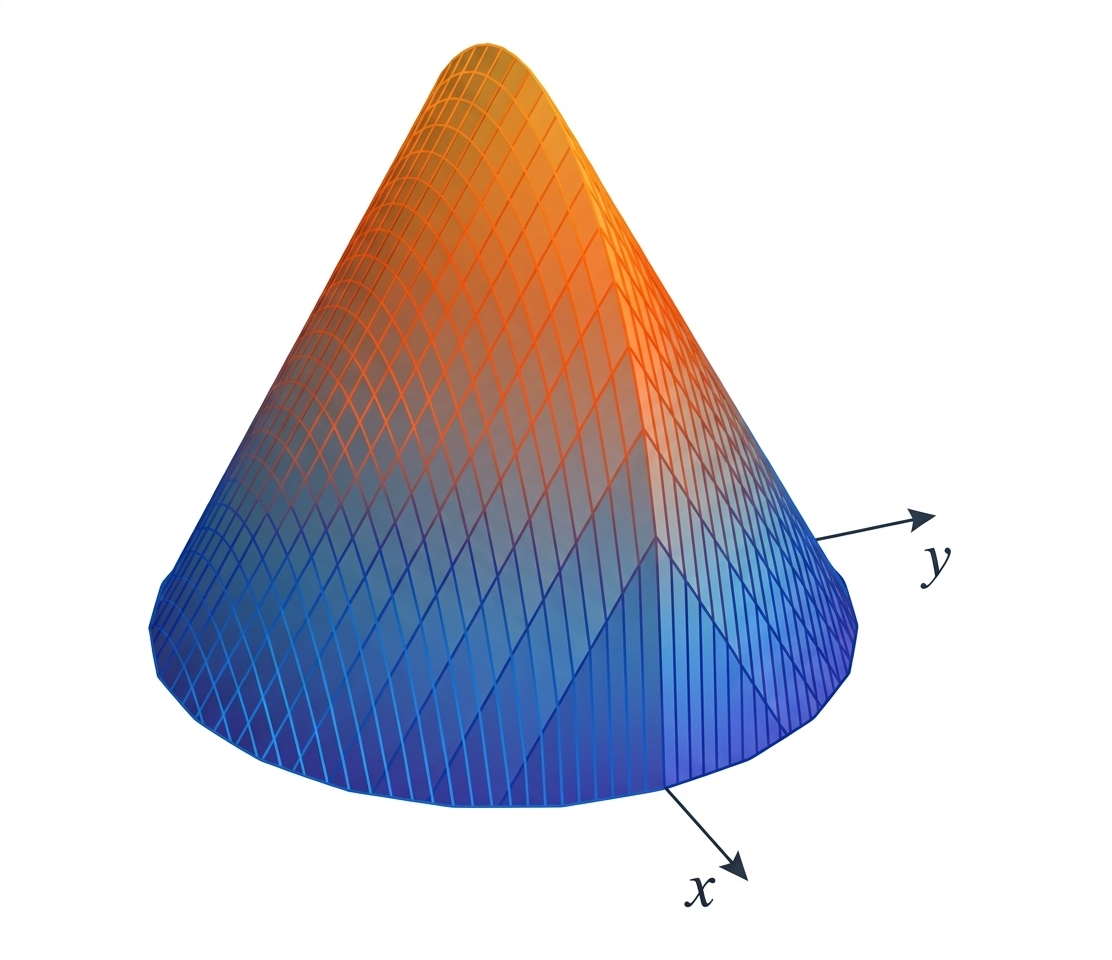
\includegraphics[width=0.5\textwidth]{images/Cau20.png}
\end{figure}
}

% --- CÂU 21 ---
\questionShortAnswer{0}{21}{Một ô tô đang chạy với vận tốc 12 m/s thì người lái xe đạp phanh. Từ thời điểm đó, ô tô chuyển động chậm dần đều với vận tốc \(v(t) = -2t + 12\) (m/s), trong đó \(t\) là khoảng thời gian được tính bằng giây, kể từ lúc bắt đầu đạp phanh. Quãng đường ô tô di chuyển được trong 10 giây cuối cùng bằng bao nhiêu? (làm tròn kết quả đến hàng đơn vị).
}

% --- CÂU 22 ---
\questionShortAnswer{0}{22}{Đơn đặt hàng của nhà máy cho một loại máy điều hoà không khí là khoảng 6000 chiếc mỗi tuần khi giá là 331 USD/chiếc và khoảng 8000 chiếc mỗi tuần khi giá là 303 USD/chiếc. Hàm cung được cho bởi \(p = 0,0275x\), trong đó \(x\) là số lượng máy điều hoà được bán với giá \(p\) USD một chiếc. Tổng thặng dư tiêu dùng và thặng dư sản xuất bằng bao nhiêu nghìn USD (giả sử hàm cầu là hàm bậc nhất)
}


\end{document}

%1C, 2B, 3A, ,4A, 5A, 6A, 7C, 8B, 9D, 10D, 11C, 12B
%13DSDD, 14DDDS, 15DDSS, 16DSSD
%17: 95 | 18: 22| 19: 305| 20: 2.31| 21: